\documentclass[]{article}
\usepackage{lmodern}
\usepackage{amssymb,amsmath}
\usepackage{ifxetex,ifluatex}
\usepackage{fixltx2e} % provides \textsubscript
\ifnum 0\ifxetex 1\fi\ifluatex 1\fi=0 % if pdftex
  \usepackage[T1]{fontenc}
  \usepackage[utf8]{inputenc}
\else % if luatex or xelatex
  \ifxetex
    \usepackage{mathspec}
  \else
    \usepackage{fontspec}
  \fi
  \defaultfontfeatures{Ligatures=TeX,Scale=MatchLowercase}
\fi
% use upquote if available, for straight quotes in verbatim environments
\IfFileExists{upquote.sty}{\usepackage{upquote}}{}
% use microtype if available
\IfFileExists{microtype.sty}{%
\usepackage{microtype}
\UseMicrotypeSet[protrusion]{basicmath} % disable protrusion for tt fonts
}{}
\usepackage[margin=1in]{geometry}
\usepackage{hyperref}
\hypersetup{unicode=true,
            pdftitle={Running the OHDSI Methods Benchmark},
            pdfauthor={Martijn J. Schuemie},
            pdfborder={0 0 0},
            breaklinks=true}
\urlstyle{same}  % don't use monospace font for urls
\usepackage{color}
\usepackage{fancyvrb}
\newcommand{\VerbBar}{|}
\newcommand{\VERB}{\Verb[commandchars=\\\{\}]}
\DefineVerbatimEnvironment{Highlighting}{Verbatim}{commandchars=\\\{\}}
% Add ',fontsize=\small' for more characters per line
\usepackage{framed}
\definecolor{shadecolor}{RGB}{248,248,248}
\newenvironment{Shaded}{\begin{snugshade}}{\end{snugshade}}
\newcommand{\AlertTok}[1]{\textcolor[rgb]{0.94,0.16,0.16}{#1}}
\newcommand{\AnnotationTok}[1]{\textcolor[rgb]{0.56,0.35,0.01}{\textbf{\textit{#1}}}}
\newcommand{\AttributeTok}[1]{\textcolor[rgb]{0.77,0.63,0.00}{#1}}
\newcommand{\BaseNTok}[1]{\textcolor[rgb]{0.00,0.00,0.81}{#1}}
\newcommand{\BuiltInTok}[1]{#1}
\newcommand{\CharTok}[1]{\textcolor[rgb]{0.31,0.60,0.02}{#1}}
\newcommand{\CommentTok}[1]{\textcolor[rgb]{0.56,0.35,0.01}{\textit{#1}}}
\newcommand{\CommentVarTok}[1]{\textcolor[rgb]{0.56,0.35,0.01}{\textbf{\textit{#1}}}}
\newcommand{\ConstantTok}[1]{\textcolor[rgb]{0.00,0.00,0.00}{#1}}
\newcommand{\ControlFlowTok}[1]{\textcolor[rgb]{0.13,0.29,0.53}{\textbf{#1}}}
\newcommand{\DataTypeTok}[1]{\textcolor[rgb]{0.13,0.29,0.53}{#1}}
\newcommand{\DecValTok}[1]{\textcolor[rgb]{0.00,0.00,0.81}{#1}}
\newcommand{\DocumentationTok}[1]{\textcolor[rgb]{0.56,0.35,0.01}{\textbf{\textit{#1}}}}
\newcommand{\ErrorTok}[1]{\textcolor[rgb]{0.64,0.00,0.00}{\textbf{#1}}}
\newcommand{\ExtensionTok}[1]{#1}
\newcommand{\FloatTok}[1]{\textcolor[rgb]{0.00,0.00,0.81}{#1}}
\newcommand{\FunctionTok}[1]{\textcolor[rgb]{0.00,0.00,0.00}{#1}}
\newcommand{\ImportTok}[1]{#1}
\newcommand{\InformationTok}[1]{\textcolor[rgb]{0.56,0.35,0.01}{\textbf{\textit{#1}}}}
\newcommand{\KeywordTok}[1]{\textcolor[rgb]{0.13,0.29,0.53}{\textbf{#1}}}
\newcommand{\NormalTok}[1]{#1}
\newcommand{\OperatorTok}[1]{\textcolor[rgb]{0.81,0.36,0.00}{\textbf{#1}}}
\newcommand{\OtherTok}[1]{\textcolor[rgb]{0.56,0.35,0.01}{#1}}
\newcommand{\PreprocessorTok}[1]{\textcolor[rgb]{0.56,0.35,0.01}{\textit{#1}}}
\newcommand{\RegionMarkerTok}[1]{#1}
\newcommand{\SpecialCharTok}[1]{\textcolor[rgb]{0.00,0.00,0.00}{#1}}
\newcommand{\SpecialStringTok}[1]{\textcolor[rgb]{0.31,0.60,0.02}{#1}}
\newcommand{\StringTok}[1]{\textcolor[rgb]{0.31,0.60,0.02}{#1}}
\newcommand{\VariableTok}[1]{\textcolor[rgb]{0.00,0.00,0.00}{#1}}
\newcommand{\VerbatimStringTok}[1]{\textcolor[rgb]{0.31,0.60,0.02}{#1}}
\newcommand{\WarningTok}[1]{\textcolor[rgb]{0.56,0.35,0.01}{\textbf{\textit{#1}}}}
\usepackage{graphicx,grffile}
\makeatletter
\def\maxwidth{\ifdim\Gin@nat@width>\linewidth\linewidth\else\Gin@nat@width\fi}
\def\maxheight{\ifdim\Gin@nat@height>\textheight\textheight\else\Gin@nat@height\fi}
\makeatother
% Scale images if necessary, so that they will not overflow the page
% margins by default, and it is still possible to overwrite the defaults
% using explicit options in \includegraphics[width, height, ...]{}
\setkeys{Gin}{width=\maxwidth,height=\maxheight,keepaspectratio}
\IfFileExists{parskip.sty}{%
\usepackage{parskip}
}{% else
\setlength{\parindent}{0pt}
\setlength{\parskip}{6pt plus 2pt minus 1pt}
}
\setlength{\emergencystretch}{3em}  % prevent overfull lines
\providecommand{\tightlist}{%
  \setlength{\itemsep}{0pt}\setlength{\parskip}{0pt}}
\setcounter{secnumdepth}{5}
% Redefines (sub)paragraphs to behave more like sections
\ifx\paragraph\undefined\else
\let\oldparagraph\paragraph
\renewcommand{\paragraph}[1]{\oldparagraph{#1}\mbox{}}
\fi
\ifx\subparagraph\undefined\else
\let\oldsubparagraph\subparagraph
\renewcommand{\subparagraph}[1]{\oldsubparagraph{#1}\mbox{}}
\fi

%%% Use protect on footnotes to avoid problems with footnotes in titles
\let\rmarkdownfootnote\footnote%
\def\footnote{\protect\rmarkdownfootnote}

%%% Change title format to be more compact
\usepackage{titling}

% Create subtitle command for use in maketitle
\providecommand{\subtitle}[1]{
  \posttitle{
    \begin{center}\large#1\end{center}
    }
}

\setlength{\droptitle}{-2em}

  \title{Running the OHDSI Methods Benchmark}
    \pretitle{\vspace{\droptitle}\centering\huge}
  \posttitle{\par}
    \author{Martijn J. Schuemie}
    \preauthor{\centering\large\emph}
  \postauthor{\par}
      \predate{\centering\large\emph}
  \postdate{\par}
    \date{2019-08-27}


\begin{document}
\maketitle

{
\setcounter{tocdepth}{2}
\tableofcontents
}
\hypertarget{introduction}{%
\section{Introduction}\label{introduction}}

When designing an observational study, there are many study designs to
choose from, and many additional choices to make, and it is often
unclear how these choices will affect the accuracy of the results.
(e.g.~If I match on propensity scores, will that lead to more or less
bias than when I stratify? What about power?) The literature contains
many papers evaluating one design choice at a time, but often with
unsatisfactory scientific rigor; typically, a method is evaluated on one
or two exemplar study from which we cannot generalize, or by using
simulations which have an unclear relationship with the real world.

This vignette describes the OHDSI Methods Benchmark for evaluating
population-level estimation methods, a benchmark that can inform on how
a particular study design and set of analysis choices perform in
general. The benchmark consists of a \textbf{gold standard} of research
hypothesis where the truth is known, and a set of \textbf{metrics} for
characterizing a methods performance when applied to the gold standard.
We distinguish between two types of tasks: (1) estimation of the average
effect of an exposure on an outcome relative to no exposure (effect
estimation), and (2) estimation of the average effect of an exposure on
an outcome relative to another exposure (comparative effect estimation).
The benchmark allows evaluation of a method on either or both tasks.

This benchmark builds on previous efforts in EU-ADR, OMOP, and the WHO,
adding the ability to evaluate methods on both tasks, and using
synthetic positive controls as real positive controls have been observed
to be problematic in the past.

\hypertarget{gold-standard}{%
\subsection{Gold standard}\label{gold-standard}}

The gold standard comprises 800 entries, with each item specifying a
target exposure, comparator exposure, outcome, nesting cohort, and true
effect size. The true effect size refers to the absolute effect of the
target on the outcome. Because the comparator is always believed to have
no effect on the outcome, the true effect size also holds for the
relative effect of the target compared to the comparator. Thus, each
entry can be used for evaluating both effect estimation and comparative
effect estimation. The nesting cohort identifies a more homogeneous
subgroup of the population and can be used to evaluate methods such as
the nested case-control design.

Of the total set, 200 entries are real negative controls with a presumed
true relative risk of 1. We select these negative controls by first
picking four diverse outcomes (acute pancreatitis, gastrointestinal
bleeding, inflammatory bowel disease, and stroke) and four diverse
exposures (ciprofloxacin, diclofenac, metformin, and sertraline). For
each of the four outcomes, we create 25 entries with target and
comparator exposures that are not believed to cause the outcome. To aid
the creation of these entries, we generate candidate lists of negative
controls for each of the four main outcomes and four main exposures
using an automated procedure, drawing on literature, product labels, and
spontaneous reports. These candidates are used to construct
target-comparator-outcome triplets where neither the target nor the
exposure causes the outcome, and the target and comparator were either
previously compared in a randomized trial per ClinicalTrials.gov, or
both had the same four-digit ATC code (same indication) but not the same
five-digit ATC code (different class). These candidates are ranked on
prevalence of the exposures and outcome and manually reviewed until 25
were approved per initial outcome or exposure. Nesting cohorts were
selected by manually reviewing the most prevalent conditions and
procedures on the first day of the target or comparator treatment.

The remaining 600 entries are positive controls, which were
automatically derived from the 200 negative controls by adding synthetic
additional outcomes during the target exposure until a desired incidence
rate ratio was achieved between before and after injection of the
synthetic outcomes. The target incidence rate ratios were 1.25, 2, and
4. To preserve (measured) confounding, predictive models were fitted for
each outcome during target exposure and used to generate probabilities
from which the synthetic outcomes were sampled.

\hypertarget{metrics}{%
\subsection{Metrics}\label{metrics}}

Once a method has been used to produce estimates for the gold standard
the following metrics are computed:

\begin{itemize}
\tightlist
\item
  \textbf{AUC}: the ability to discriminate between positive controls
  and negative controls.
\item
  \textbf{Coverage}: how often the true effect size is within the 95\%
  confidence interval.
\item
  \textbf{Mean precision}: Precision is computed as 1 / (standard
  error)2, higher precision means narrower confidence intervals. We use
  the geometric mean to account for the skewed distribution of the
  precision.
\item
  \textbf{Mean squared error} (MSE): Mean squared error between the log
  of the effect size point-estimate and the log of the true effect size.
\item
  \textbf{Type 1 error}: For negative controls, how often was the null
  rejected (at alpha = 0.05). This is equivalent to the false positive
  rate and 1 - specificity.
\item
  \textbf{Type 2 error}: For positive controls, how often was the null
  not rejected (at alpha = 0.05). This is equivalent to the false
  negative rate and 1 - sensitivity.
\item
  \textbf{Non-estimable}: For how many of the controls was the method
  unable to produce an estimate? There can be various reasons why an
  estimate cannot be produced, for example because there were no
  subjects left after propensity score matching, or because no subjects
  remained having the outcome.
\end{itemize}

The Benchmark computes these metrics both overall, as well as stratified
by true effect size, by each of the four initial outcomes and four
initial exposures, and by amount of data as reflected by the minimum
detectable relative risk (MDRR). When a method cannot estimate an
effect, it returns an estimate of 1 with an infinite confidence
interval.

In prior work we described a method for empirically calibrating p-values
and confidence intervals. Briefly, empirical calibration estimates a
systematic error distribution based on the estimates produced for the
negative and positive controls. This systematic error is then taken into
consideration, in addition to the random error, when computing the
confidence interval and p-value. We therefore also report the
performance metrics listed above after calibration, using a
leave-one-out approach: for each control the error distributions are
fitted on all controls except the control being calibrated and its
siblings. By siblings we mean the set of a negative control and the
positive controls derived from that negative control.

\hypertarget{running-the-benchmark}{%
\section{Running the benchmark}\label{running-the-benchmark}}

This section will describe how to run methods against the benchmark on a
particular observational healthcare database. The database needs to
conform to the OMOP Common Data Model (CDM).

\hypertarget{specifying-locations-on-the-server-and-local-file-system}{%
\subsection{Specifying locations on the server and local file
system}\label{specifying-locations-on-the-server-and-local-file-system}}

We need to specify the following locations on the database server:

\begin{itemize}
\tightlist
\item
  The database schema containing the observational healthcare data in
  \textbf{CDM} format. Only read access is required to this schema.
\item
  A database schema and table name where \textbf{outcome cohorts} can be
  instantiated. Write access is required to this schema.
\item
  A database schema and table name where \textbf{nesting cohorts} can be
  instantiated. Write access is required to this schema.
\item
  \emph{On Oracle only}: a schema where \textbf{temporary tables} can be
  created. Write access is required to this schema. This is required
  since Oracle doesn't fully support temp tables like other database
  platforms.
\end{itemize}

We also need to specify on the local file system:

\begin{itemize}
\tightlist
\item
  An \textbf{output folder} where all intermediary and final results can
  be written. This should not be a network drive, since that would
  severely slow down the analyses.
\end{itemize}

Below is example code showing we specify how to connect to the database
server, and the various required locations. \texttt{MethodEvaluation}
uses the \texttt{DatabaseConnector} package, which provides the
\texttt{createConnectionDetails} function. Type
\texttt{?createConnectionDetails} for the specific settings required for
the various database management systems (DBMS).

\begin{Shaded}
\begin{Highlighting}[]
\KeywordTok{library}\NormalTok{(MethodEvaluation)}
\NormalTok{connectionDetails <-}\StringTok{ }\KeywordTok{createConnectionDetails}\NormalTok{(}\DataTypeTok{dbms =} \StringTok{"postgresql"}\NormalTok{, }
                                             \DataTypeTok{server =} \StringTok{"localhost/ohdsi"}\NormalTok{, }
                                             \DataTypeTok{user =} \StringTok{"joe"}\NormalTok{, }
                                             \DataTypeTok{password =} \StringTok{"supersecret"}\NormalTok{)}

\NormalTok{cdmDatabaseSchema <-}\StringTok{ "my_cdm_data"}
\NormalTok{oracleTempSchema <-}\StringTok{ }\OtherTok{NULL}
\NormalTok{outcomeDatabaseSchema <-}\StringTok{ "scratch"}
\NormalTok{outcomeTable <-}\StringTok{ "ohdsi_outcomes"}
\NormalTok{nestingCohortDatabaseSchema <-}\StringTok{ "scratch"}
\NormalTok{nestingCohortTable <-}\StringTok{ "ohdsi_nesting_cohorts"}
\NormalTok{outputFolder <-}\StringTok{ "/home/benchmarkOutput"}
\NormalTok{cdmVersion <-}\StringTok{ "5"}
\end{Highlighting}
\end{Shaded}

Note that for Microsoft SQL Server, database schemas need to specify
both the database and the schema, so for example
\texttt{cdmDatabaseSchema\ \textless{}-\ "my\_cdm\_data.dbo"}.

\hypertarget{creating-all-necessary-cohorts}{%
\subsection{Creating all necessary
cohorts}\label{creating-all-necessary-cohorts}}

In order to run our population-level effect estimation method, we will
need to identify the exposures and outcomes of interest. To identify
exposures we will simlpy use the predefined exposure eras in the
\texttt{drug\_era} table in the CDM. However, for the outcomes custom
cohorts need to be generated. In addition, some methods such as the
nested case-control design require nesting cohorts to be defined. The
negative control outcome and nesting cohorts can be generated using the
following command:

\begin{Shaded}
\begin{Highlighting}[]
\KeywordTok{createReferenceSetCohorts}\NormalTok{(}\DataTypeTok{connectionDetails =}\NormalTok{ connectionDetails,}
                          \DataTypeTok{oracleTempSchema =}\NormalTok{ oracleTempSchema,}
                          \DataTypeTok{cdmDatabaseSchema =}\NormalTok{ cdmDatabaseSchema,}
                          \DataTypeTok{outcomeDatabaseSchema =}\NormalTok{ outcomeDatabaseSchema,}
                          \DataTypeTok{outcomeTable =}\NormalTok{ outcomeTable,}
                          \DataTypeTok{nestingDatabaseSchema =}\NormalTok{ nestingCohortDatabaseSchema,}
                          \DataTypeTok{nestingTable =}\NormalTok{ nestingCohortTable,}
                          \DataTypeTok{referenceSet =} \StringTok{"ohdsiMethodsBenchmark"}\NormalTok{)}
\end{Highlighting}
\end{Shaded}

This will automatically create the outcome and nesting cohort tables,
and populate them.

The nest step is to create the positive controls. These are generated by
taking the negative controls, and adding synthetic outcomes during
exposed time to achieve predefined relative risks greater than one. The
synthetic outcomes are sampled based on models that are fitted for each
negative control outcome, using predictors extracted from the data.
These positive control outcomes are added to the outcome table.

\begin{Shaded}
\begin{Highlighting}[]
\KeywordTok{synthesizeReferenceSetPositiveControls}\NormalTok{(}\DataTypeTok{connectionDetails =}\NormalTok{ connectionDetails,}
                                       \DataTypeTok{oracleTempSchema =}\NormalTok{ oracleTempSchema,}
                                       \DataTypeTok{cdmDatabaseSchema =}\NormalTok{ cdmDatabaseSchema,}
                                       \DataTypeTok{outcomeDatabaseSchema =}\NormalTok{ outcomeDatabaseSchema,}
                                       \DataTypeTok{outcomeTable =}\NormalTok{ outcomeTable,}
                                       \DataTypeTok{maxCores =} \DecValTok{10}\NormalTok{,}
                                       \DataTypeTok{workFolder =}\NormalTok{ outputFolder,}
                                       \DataTypeTok{summaryFileName =} \KeywordTok{file.path}\NormalTok{(outputFolder, }
                                                                   \StringTok{"allControls.csv"}\NormalTok{),}
                                       \DataTypeTok{referenceSet =} \StringTok{"ohdsiMethodsBenchmark"}\NormalTok{)}
\end{Highlighting}
\end{Shaded}

Fitting the outcome models can take a while. It is recommend to set the
\texttt{maxCores} argument to the number of CPU cores available in the
machine to speed up the process. Note that at the end, a file will be
created called \emph{allControls.csv} in the output folder containing
the information on the controls:

\begin{Shaded}
\begin{Highlighting}[]
\NormalTok{allControls <-}\StringTok{ }\KeywordTok{read.csv}\NormalTok{(}\KeywordTok{file.path}\NormalTok{(outputFolder, }\StringTok{"allControls.csv"}\NormalTok{))}
\KeywordTok{head}\NormalTok{(allControls)}
\end{Highlighting}
\end{Shaded}

\begin{verbatim}
#>  outcomeId comparatorId targetId targetName comparatorName nestingId                  nestingName        outcomeName             type targetEffectSize trueEffectSize trueEffectSizeFirstExposure oldOutcomeId mdrrTarget
#> 1         1      1105775  1110942 omalizumab  Aminophylline  37203741 Bronchospasm and obstruction Acute pancreatitis Exposure control                1              1                           1            1   1.421960
#> 2         1      1110942  1140088 Dyphylline     omalizumab  37203741 Bronchospasm and obstruction Acute pancreatitis Exposure control                1              1                           1            1   1.420173
#> 3         1      1136422   943634 epinastine levocetirizine  36009773            Rhinitis allergic Acute pancreatitis Exposure control                1              1                           1            1   1.217681
#> 4         1      1315865 40163718  prasugrel   fondaparinux  37622411              Phlebosclerosis Acute pancreatitis Exposure control                1              1                           1            1   1.196514
#> 5         1      1315865  1350310 cilostazol   fondaparinux  37622411              Phlebosclerosis Acute pancreatitis Exposure control                1              1                           1            1   1.233415
#> 6         1      1336926  1311276 vardenafil      tadalafil  36919202           Sexual dysfunction Acute pancreatitis Exposure control                1              1                           1            1   1.097112
#>   mdrrComparator
#> 1       1.177202
#> 2       1.421960
#> 3       1.085877
#> 4       1.278911
#> 5       1.278911
#> 6       1.060737
\end{verbatim}

\hypertarget{running-the-method-to-evaluate}{%
\subsection{Running the method to
evaluate}\label{running-the-method-to-evaluate}}

Now that we have the controls in place, we can run the method we would
like to evaluate. Here we will run the \texttt{SelfControlledCohort}
package which implements the Self-Controlled Cohort (SCC) design. We
first will first define some SCC analysis settings to evaluate. Here we
define two analysis settings, one using the length of exposure as the
time-at-risk, and one using the first 30 days after exposure start as
the time-at-risk:

\begin{Shaded}
\begin{Highlighting}[]
\KeywordTok{library}\NormalTok{(SelfControlledCohort)}
\NormalTok{runSccArgs1 <-}\StringTok{ }\KeywordTok{createRunSelfControlledCohortArgs}\NormalTok{(}\DataTypeTok{addLengthOfExposureExposed =} \OtherTok{TRUE}\NormalTok{,}
                                                 \DataTypeTok{riskWindowStartExposed =} \DecValTok{0}\NormalTok{,}
                                                 \DataTypeTok{riskWindowEndExposed =} \DecValTok{0}\NormalTok{,}
                                                 \DataTypeTok{riskWindowEndUnexposed =} \DecValTok{-1}\NormalTok{,}
                                                 \DataTypeTok{addLengthOfExposureUnexposed =} \OtherTok{TRUE}\NormalTok{,}
                                                 \DataTypeTok{riskWindowStartUnexposed =} \DecValTok{-1}\NormalTok{,}
                                                 \DataTypeTok{washoutPeriod =} \DecValTok{365}\NormalTok{)}

\NormalTok{sccAnalysis1 <-}\StringTok{ }\KeywordTok{createSccAnalysis}\NormalTok{(}\DataTypeTok{analysisId =} \DecValTok{1}\NormalTok{,}
                                  \DataTypeTok{description =} \StringTok{"Length of exposure"}\NormalTok{,}
                                  \DataTypeTok{runSelfControlledCohortArgs =}\NormalTok{ runSccArgs1)}

\NormalTok{runSccArgs2 <-}\StringTok{ }\KeywordTok{createRunSelfControlledCohortArgs}\NormalTok{(}\DataTypeTok{addLengthOfExposureExposed =} \OtherTok{FALSE}\NormalTok{,}
                                                 \DataTypeTok{riskWindowStartExposed =} \DecValTok{0}\NormalTok{,}
                                                 \DataTypeTok{riskWindowEndExposed =} \DecValTok{30}\NormalTok{,}
                                                 \DataTypeTok{riskWindowEndUnexposed =} \DecValTok{-1}\NormalTok{,}
                                                 \DataTypeTok{addLengthOfExposureUnexposed =} \OtherTok{FALSE}\NormalTok{,}
                                                 \DataTypeTok{riskWindowStartUnexposed =} \DecValTok{-30}\NormalTok{,}
                                                 \DataTypeTok{washoutPeriod =} \DecValTok{365}\NormalTok{)}

\NormalTok{sccAnalysis2 <-}\StringTok{ }\KeywordTok{createSccAnalysis}\NormalTok{(}\DataTypeTok{analysisId =} \DecValTok{2}\NormalTok{,}
                                  \DataTypeTok{description =} \StringTok{"30 days of each exposure"}\NormalTok{,}
                                  \DataTypeTok{runSelfControlledCohortArgs =}\NormalTok{ runSccArgs2)}
\NormalTok{sccAnalysisList <-}\StringTok{ }\KeywordTok{list}\NormalTok{(sccAnalysis1, sccAnalysis2)}
\end{Highlighting}
\end{Shaded}

Next, we specify all exposure-outcome pairs we want to apply the SCC
design to. Note that we only use the \texttt{targetId} and
\texttt{outcomeId} fields of the controls, because the SCC design can
only be used for effect estimation, and does not support nesting:

\begin{Shaded}
\begin{Highlighting}[]
\NormalTok{allControls <-}\StringTok{ }\KeywordTok{read.csv}\NormalTok{(}\KeywordTok{file.path}\NormalTok{(outputFolder , }\StringTok{"allControls.csv"}\NormalTok{))}
\NormalTok{eos <-}\StringTok{ }\KeywordTok{list}\NormalTok{()}
\ControlFlowTok{for}\NormalTok{ (i }\ControlFlowTok{in} \DecValTok{1}\OperatorTok{:}\KeywordTok{nrow}\NormalTok{(allControls)) \{}
\NormalTok{  eos[[}\KeywordTok{length}\NormalTok{(eos) }\OperatorTok{+}\StringTok{ }\DecValTok{1}\NormalTok{]] <-}\StringTok{ }\KeywordTok{createExposureOutcome}\NormalTok{(}\DataTypeTok{exposureId =}\NormalTok{ allControls}\OperatorTok{$}\NormalTok{targetId[i],}
                                                  \DataTypeTok{outcomeId =}\NormalTok{ allControls}\OperatorTok{$}\NormalTok{outcomeId[i])}
\NormalTok{\}}
\end{Highlighting}
\end{Shaded}

Then, we run the SCC method. The following command will execute the SCC
with the specified analysis settings against the exposure-outcome pairs:

\begin{Shaded}
\begin{Highlighting}[]
\NormalTok{sccResult <-}\StringTok{ }\KeywordTok{runSccAnalyses}\NormalTok{(}\DataTypeTok{connectionDetails =}\NormalTok{ connectionDetails,}
                            \DataTypeTok{cdmDatabaseSchema =}\NormalTok{ cdmDatabaseSchema,}
                            \DataTypeTok{oracleTempSchema =}\NormalTok{ oracleTempSchema,}
                            \DataTypeTok{exposureTable =} \StringTok{"drug_era"}\NormalTok{,}
                            \DataTypeTok{outcomeDatabaseSchema =}\NormalTok{ outcomeDatabaseSchema,}
                            \DataTypeTok{outcomeTable =}\NormalTok{ outcomeTable,}
                            \DataTypeTok{sccAnalysisList =}\NormalTok{ sccAnalysisList,}
                            \DataTypeTok{exposureOutcomeList =}\NormalTok{ eos,}
                            \DataTypeTok{outputFolder =}\NormalTok{ outputFolder)}
\NormalTok{sccSummary <-}\StringTok{ }\KeywordTok{summarizeAnalyses}\NormalTok{(sccResult, outputFolder)}
\KeywordTok{write.csv}\NormalTok{(sccSummary, }\KeywordTok{file.path}\NormalTok{(outputFolder, }\StringTok{"sccSummary.csv"}\NormalTok{), }\DataTypeTok{row.names =} \OtherTok{FALSE}\NormalTok{)}
\end{Highlighting}
\end{Shaded}

This produces a file called \emph{sccSummary.csv} which contains the
effect size estimates for each analysisId-exposureId-outcomeId
combination.

\hypertarget{packaging-the-evaluation-results}{%
\subsection{Packaging the evaluation
results}\label{packaging-the-evaluation-results}}

Now that we have the estimates, we need to feed them back into the
\texttt{MethodEvaluation} package. To do that we need to create two data
frames, one specifying the effect size estimates, the other providing
details on the various analyses.

First, we specify the estimates:

\begin{Shaded}
\begin{Highlighting}[]
\NormalTok{estimates <-}\StringTok{ }\KeywordTok{readRDS}\NormalTok{(}\KeywordTok{file.path}\NormalTok{(outputFolder, }\StringTok{"sccSummary.csv"}\NormalTok{))}
\NormalTok{estimates <-}\StringTok{ }\KeywordTok{data.frame}\NormalTok{(}\DataTypeTok{analysisId =}\NormalTok{ estimates}\OperatorTok{$}\NormalTok{analysisId,}
                        \DataTypeTok{targetId =}\NormalTok{ estimates}\OperatorTok{$}\NormalTok{exposureId,}
                        \DataTypeTok{outcomeId =}\NormalTok{ estimates}\OperatorTok{$}\NormalTok{outcomeId,}
                        \DataTypeTok{logRr =}\NormalTok{ estimates}\OperatorTok{$}\NormalTok{logRr,}
                        \DataTypeTok{seLogRr =}\NormalTok{ estimates}\OperatorTok{$}\NormalTok{seLogRr,}
                        \DataTypeTok{ci95Lb =}\NormalTok{ estimates}\OperatorTok{$}\NormalTok{irrLb95,}
                        \DataTypeTok{ci95Ub =}\NormalTok{ estimates}\OperatorTok{$}\NormalTok{irrUb95)}
\KeywordTok{head}\NormalTok{(estimates)}
\end{Highlighting}
\end{Shaded}

\begin{verbatim}
#>   analysisId targetId outcomeId      logRr   seLogRr    ci95Lb    ci95Ub
#> 1          1  1110942         1 -1.5000000        NA        NA 13.177433
#> 2          1  1140088         1         NA        NA        NA        NA
#> 3          1   943634         1         NA        NA        NA        NA
#> 4          1 40163718         1 -0.4054651 0.6926191 0.1479317  2.234489
#> 5          1  1350310         1 -0.2876821 0.7038381 0.1642789  2.592973
#> 6          1  1311276         1 -0.1823216 0.5451585 0.2651910  2.247182
\end{verbatim}

Next, we create the analysis reference:

\begin{Shaded}
\begin{Highlighting}[]
\CommentTok{# Create a reference of the analysis settings:}
\NormalTok{analysisRef <-}\StringTok{ }\KeywordTok{data.frame}\NormalTok{(}\DataTypeTok{method =} \StringTok{"SelfControlledCohort"}\NormalTok{,}
                          \DataTypeTok{analysisId =} \KeywordTok{c}\NormalTok{(}\DecValTok{1}\NormalTok{, }\DecValTok{2}\NormalTok{),}
                          \DataTypeTok{description =} \KeywordTok{c}\NormalTok{(}\StringTok{"Length of exposure"}\NormalTok{, }
                                          \StringTok{"30 days of each exposure"}\NormalTok{),}
                          \DataTypeTok{details =} \StringTok{""}\NormalTok{,}
                          \DataTypeTok{comparative =} \OtherTok{FALSE}\NormalTok{,}
                          \DataTypeTok{nesting =} \OtherTok{FALSE}\NormalTok{,}
                          \DataTypeTok{firstExposureOnly =} \OtherTok{FALSE}\NormalTok{)}
\KeywordTok{head}\NormalTok{(analysisRef)}
\end{Highlighting}
\end{Shaded}

\begin{verbatim}
#>                 method analysisId              description details
#> 1 SelfControlledCohort          1       Length of exposure        
#> 2 SelfControlledCohort          2 30 days of each exposure        
#>   comparative nesting firstExposureOnly
#> 1       FALSE   FALSE             FALSE
#> 2       FALSE   FALSE             FALSE
\end{verbatim}

Finally, we supply these two data frames, together with the data frame
with controls to the \texttt{packageOhdsiBenchmarkResults} function:

\begin{Shaded}
\begin{Highlighting}[]
\NormalTok{allControls <-}\StringTok{ }\KeywordTok{read.csv}\NormalTok{(}\KeywordTok{file.path}\NormalTok{(outputFolder , }\StringTok{"allControls.csv"}\NormalTok{))}
\KeywordTok{packageOhdsiBenchmarkResults}\NormalTok{(}\DataTypeTok{estimates =}\NormalTok{ estimates,}
                             \DataTypeTok{controlSummary =}\NormalTok{ allControls,}
                             \DataTypeTok{analysisRef =}\NormalTok{ analysisRef,}
                             \DataTypeTok{databaseName =}\NormalTok{ databaseName,}
                             \DataTypeTok{exportFolder =} \KeywordTok{file.path}\NormalTok{(outputFolder, }\StringTok{"export"}\NormalTok{))}
\end{Highlighting}
\end{Shaded}

This will generate two CSV files in the export folder. Results from
different methods and databases can all be written to the same export
folder.

\hypertarget{computing-metrics}{%
\subsection{Computing metrics}\label{computing-metrics}}

There are two ways to view the method's performance metrics: using a
Shiny app, and by generating a data frame.

\hypertarget{using-the-shiny-app}{%
\subsubsection{Using the Shiny app}\label{using-the-shiny-app}}

Run the follow command to launch the Shiny app and view the metrics:

\begin{Shaded}
\begin{Highlighting}[]
\NormalTok{exportFolder <-}\StringTok{ }\KeywordTok{file.path}\NormalTok{(outputFolder, }\StringTok{"export"}\NormalTok{)}
\KeywordTok{launchMethodEvaluationApp}\NormalTok{(exportFolder)}
\end{Highlighting}
\end{Shaded}

This will launch a Shiny app as shown in Figure 1.

\begin{figure}
\centering
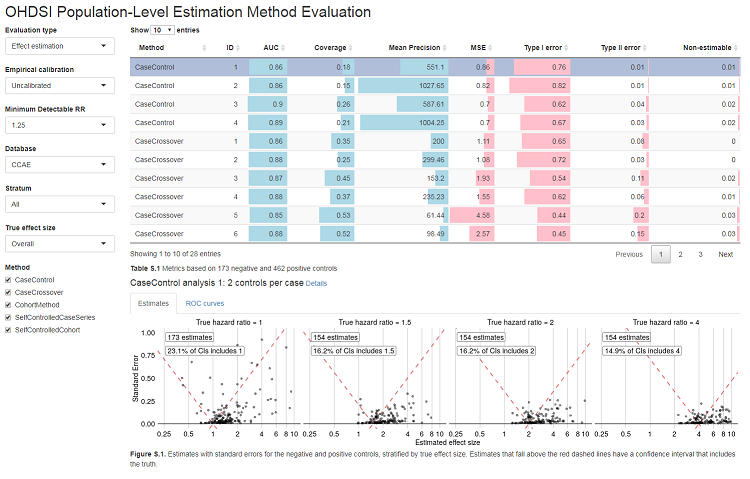
\includegraphics{shiny.png}
\caption{Method Benchmark Shiny app}
\end{figure}

Note that the export folder can hold results from multiple methods and
multiple databases.

\hypertarget{generating-a-data-frame}{%
\subsubsection{Generating a data frame}\label{generating-a-data-frame}}

Alternatively, we can output the metrics to a data frame:

\begin{Shaded}
\begin{Highlighting}[]
\NormalTok{exportFolder <-}\StringTok{ }\KeywordTok{file.path}\NormalTok{(outputFolder, }\StringTok{"export"}\NormalTok{)}
\NormalTok{metrics <-}\StringTok{ }\KeywordTok{computeOhdsiBenchmarkMetrics}\NormalTok{(exportFolder, }
                                        \DataTypeTok{mdrr =} \FloatTok{1.25}\NormalTok{, }
                                        \DataTypeTok{stratum =} \StringTok{"All"}\NormalTok{, }
                                        \DataTypeTok{trueEffectSize =} \StringTok{"Overall"}\NormalTok{, }
                                        \DataTypeTok{calibrated =} \OtherTok{FALSE}\NormalTok{, }
                                        \DataTypeTok{comparative =} \OtherTok{FALSE}\NormalTok{)}
\KeywordTok{head}\NormalTok{(metrics)}
\end{Highlighting}
\end{Shaded}

\begin{verbatim}
#>    database               method analysisId                                           description  auc coverage   meanP  mse type1 type2 nonEstimable
#> 1     CCAE SelfControlledCohort          1                    Length of exposure 0.89     0.21 1048.97 0.30  0.66  0.08         0.01
#> 2     CCAE SelfControlledCohort          2                        30 days of each exposure 0.87     0.41  422.25 0.14  0.55  0.11         0.00
\end{verbatim}

See \texttt{?computeOhdsiBenchmarkMetrics} for information on the
various arguments.


\end{document}
